\documentclass{article}
\usepackage{arxiv}
\usepackage[utf8]{inputenc} % allow utf-8 input
\usepackage[T1]{fontenc}    % use 8-bit T1 fonts
\usepackage{hyperref}       % hyperlinks
\usepackage{url}            % simple URL typesetting
\usepackage{booktabs}       % professional-quality tables
\usepackage{amsfonts}       % blackboard math symbols
\usepackage{nicefrac}       % compact symbols for 1/2, etc.
\usepackage{microtype}      % microtypography
\usepackage{lipsum}		% Can be removed after putting your text content
\usepackage{graphicx}
\usepackage{natbib}
\usepackage{doi}

\title{Retrieval-Based Chatbots}

\date{January 30, 2021}	% Here you can change the date presented in the paper title

\author{ {
\hspace{1mm}Huchi} \\
Natural Language Processing Research Group\\
	Department of Computer Science\\
	NanJing University\\
	\texttt{huchiq@gmail.com} \\
}

\renewcommand{\shorttitle}{\textit{NLP} Report}

\hypersetup{
pdftitle={A report for the NJU NLP course},
pdfsubject={q-bio.NC, q-bio.QM},
pdfauthor={Renjie Wang},
pdfkeywords={Chatbots, Dialog System, Conversational AI, Response Selection},
}

\begin{document}
\maketitle

\begin{abstract}
In this article, we mainly elaborated retrieval-based dialog system. First, we introduce the formal problem definition of dialogue system and its core concept definition. We give the structure of the retrieval-based dialogue system, and describe in detail the two parts of it: 1) the fine-grained Ranking system and 2) the coarse-grained candidate set generation system. In the experimental part, we give the results of our experiment and optimize the performance of the candidate set generation system through the faiss library. Finally, we analyze and summarize the shortcoming and future trends of retrieval-based dialog system.
\end{abstract}

\keywords{Chatbots \and Dialog System \and Conversational AI \and Response Selection}

\section{Introduction}
Building an intelligent chatbot that can have a coherent and interesting conversation with people like human beings is a necessary way to realize the Turing Test proposed by \cite{turing2009computing}. This also has been a long-standing goal of artificial intelligence (AI).

Dialog systems such as Microsoft XiaoIce designed by \cite{zhou2020design}, have attracted millions of users and can converse with users on a wide variety of topics for hours. Though XiaoIce has been suspending service now, there are more and more mature chatbots entering the commercial stage like Facebook ChatBots, Google Allo and so on. Although these intelligent chatbots can provide a good user experience, there are still many unsolved problems, such as the inability to simultaneously meet the picture and text interaction, the lack of common sense reasoning ability with common knowledge, and uncontrollable generated content and others. \par

In order to answer a given conversation by generating or retrieving a response, the conversation system must automatically understand the implicit structure of the conversation in addition to describing the discussion part of the problem and solution meanwhile. However, such implicit information is difficult to capture. Based on neural deep learning technique, we can't control the generated content from a deep learning generating model. So in this article, we only talk about the retrieval technique whose response is controllable, which won't produce anti-social or anti-human speech. In particular,  the response can be selected from a candidate set which can be prescreened and revised with desired qualities such as fluency and diversity. However, when we need to build a better retrieval-based dialogue system, more challenges will arise, such as how to speed up time for retrieving to meet industrial needs. \par

Despite the recent success of neural approaches to natural language processing and conversational AI, building a better chatbot still faces three challenges as \cite{huang2020challenges} talked: semantics, consistency and interactiveness. First, semantics requires a dialog system to understand the intention of the dialog and identify users’ sentiment and social requires continuously. Second, consistency requires the system containing a consistent personality to win users’ trust and gain their long-term confidence. Third, interactiveness refers to the system’s ability to make interpersonal responses to meet particular social needs such as entertainment, conforming and advising. \par

Recently, more efforts have been made to design better architectures such as DialogXL(\cite{shen2020dialogxl}) or to better learn the match between dialog context and candidate responses, while relatively little effort has been devoted to deploying an available production model in real environments. \par

In this paper, we explore and evaluate retrieval-based chatbots. We not only pay attention to the performance indicators of the model, but also pay attention to the inference speed of the model, which is the practical application limitation in industrial scenarios. The rest of the article is structured as follows: In Section \ref{section2}, we give the brief definition of the retrieval-based dialog and important concepts involved. In Section \ref{section3}, we describe the general architecture of the dialogue system and the NLP(Natural Language Process) algorithm involved in. In Section 4, we analyze the shortcomings of existing methods and give our own hypothetical methods and part of experimental results. In Section 5, we summarize and give the possible development trend of the current dialog system.

\section{Core Definition}
\label{section2}

Before explaining dialog systems, it is important to understand the definition of dialog and the properties and structure of dialog. One dialog can be viewed as a succession of utterances (dialog turns) between two or multiple parties who have goals and intentions to talk with others.

Dialog systems need to be able to understand the context of the conversation, identify the intentions and the goals of the speaker and produce a coherent response. There are three key concepts of dialogue. First, in the literature, the term context may refer to the preceding utterances (dialog turns). Second, the speaker intentions and goals are usually implicit and encoded inside the utterances. Instead of telling the hearer what to do, the speaker may just express his goals, and expect a response that meets their goals. The third concept is the dialogue cohesion. Cohesion in dialog means that the response need to be consistent with the context so that makes a text semantically meaningful.

\subsection{Problem Formalization}

 At the heart of a dialog system is a response generation engine that gets user input at $t$-th dialog turn $X_{t}=x_{1}^{t} x_{2}^{t} \cdots x_{n}^{t}$ and dialog context $S_{t}$  and generates response $Y_{t}=y_{1}^{t} y_{2}^{t} \cdots y_{m}^{t}$ as

\begin{equation}
\hat{Y}_{t}={\arg \max }_{Y \in \Omega} \mathcal{G}_{\theta}\left(Y \mid X_{t}, S_{t}\right)
\end{equation}

where $\Omega$ is the set of all candidate responses, $\mathcal{G}_{\theta}$ is a learned model of scoring candidate responses, parameterized by $\theta$, and use argmax  search algorithm to find the best one with the highest score among all candidates. \par

Here we simply think the retrieval-based dialog system as a multi-turn response selection problem. Suppose that we have a data set $\mathcal{D}=\left\{\left(y_{i}, s_{i}, r_{i}\right)\right\}_{i=1}^{N},$ where $s_{i}$ is a conversation context, $r_{i}$ is a response candidate, and $y_{i} \in\{0,1\}$ is a label. $s_{i}=\left\{u_{i, 1}, \ldots, u_{i, n_{i}}\right\}$ where $\left\{u_{i, k}\right\}_{k=1}^{n_{i}}$ are utterances. $y_{i}=1$ if $r_{i}$ is a proper response to $s_{i}$, otherwise $y_{i}=0 .$ Our goal is to learn a matching model $g(\cdot, \cdot)$ with $\mathcal{D},$ and thus for any new context-response pair $(s, r), g(s, r)$ measures their matching degree. According to $g(s, r),$ we can rank candidates for $s$ and select a proper one as its response.

In retrieval-based methods, the search space $\Omega$ is obtained by retrieving candidate responses from a pre-collected human conversational dataset consisting of input-context-response pairs. $\mathcal{G}_{\theta}\left(Y \mid X_{t}, S_{t}\right)$ is implemented as a matching and ranking function that scores the relevance of each candidate given $X_{t}$ and $S_{t} .$

\subsection{Metric}

To measure the performance of those selection modules in real scenarios, there are several custom evaluation metrics, we mainly divide into two parts: match scores metrics, inference speed metrics.

For match scores metrics, Precision and Recall are binary metrics used to evaluate systems with binary output such as binary classifiers. In the case of retrieval-based dialogue systems, the output of the system is a ranked list of responses which is similar to recommendation systems and Information Retrieval System. Here we need to evaluate the ability of the system to rank the ground-truth responses among the k best-ranked responses. we list the most common retrieval metrics widely used in evaluating retrieval-based dialogue systems:

\paragraph{Recallk@K} It calculates the proportion of relevant responses that are in the top-k responses for a K size candidate set, it computed as follows:

\begin{equation}
    Recallk@K = \frac{\sum_{i=1}^{k} item \quad top_i\quad is \quad relevant \quad  responses}{\sum_{i=1}^{K} 1}
\end{equation}

\paragraph{Precision@k} It calculates the true proportion of relevant responses that are in the selected top-k list, it computed as follows, and the most common is Precision@1:

\begin{equation}
    Precision@k = \frac{\sum_{i=1}^{k} item \quad top_i\quad is \quad relevant \quad  responses}{\sum_{i=1}^{k} 1}
\end{equation}

\paragraph{MAP} (Mean Average Precision) is the average of Average Precision over a set of queries. AP is the average of precision values at the ranks where relevant responses are found.


\begin{equation}
\mathbf{MAP}=\frac{1}{|S|} \sum_{i=1}^{|S|} \frac{1}{m_{i}} \sum_{k=1}^{m_{i}} \text { Precision@k } \times [top_k\quad is \quad relevant]
\end{equation}

Where $S$ is the set of contexts, $m_i$ is the total number of ground-truth responses of the context $i$ and $[top_k\quad is \quad relevant]$ is an indicator function equal to 1 if the response at rank $k$ is relevant, 0 otherwise.

\paragraph{MRR} (Mean Reciprocal Rank) is the average of the reciprocal of the ranks at which the ground-truth responses were ranked for all the contexts. Suppose that we have one ground-truth response, its reciprocal rank is $1/i$ if it ranks $i$-th. The MRR is computed as follows:

\begin{equation}
\mathrm{MRR}=\frac{1}{|S|} \sum_{i=1}^{|S|} \frac{1}{\operatorname{rank}_{i}}
\end{equation}

Where $S$ is the set of contexts and $rank_i$ refers to the rank of the first retrieved ground-truth response for the $i$-t context. Besides, sometime we also can calculate $rank_i$ as the mean average of all retrieved ground-truth response for the $i$-th context.

These evaluation metrics used for retrieval-based dialogue systems simply check whether the ground-truth response appear in the ranked list, which seems similar to the metrics in Recommend System. But these metrics can't take the semantic between the selected list and the query context into consideration. If we want to do this, a common metric is human evaluation which is the most reliable metric to measure the performance of dialog systems. Meanwhile, infer time cost is also a core metric in a real production, which directly influences users' experience.

\begin{figure}[htb]
\caption{Architecture of Dialog System}
	\centering
	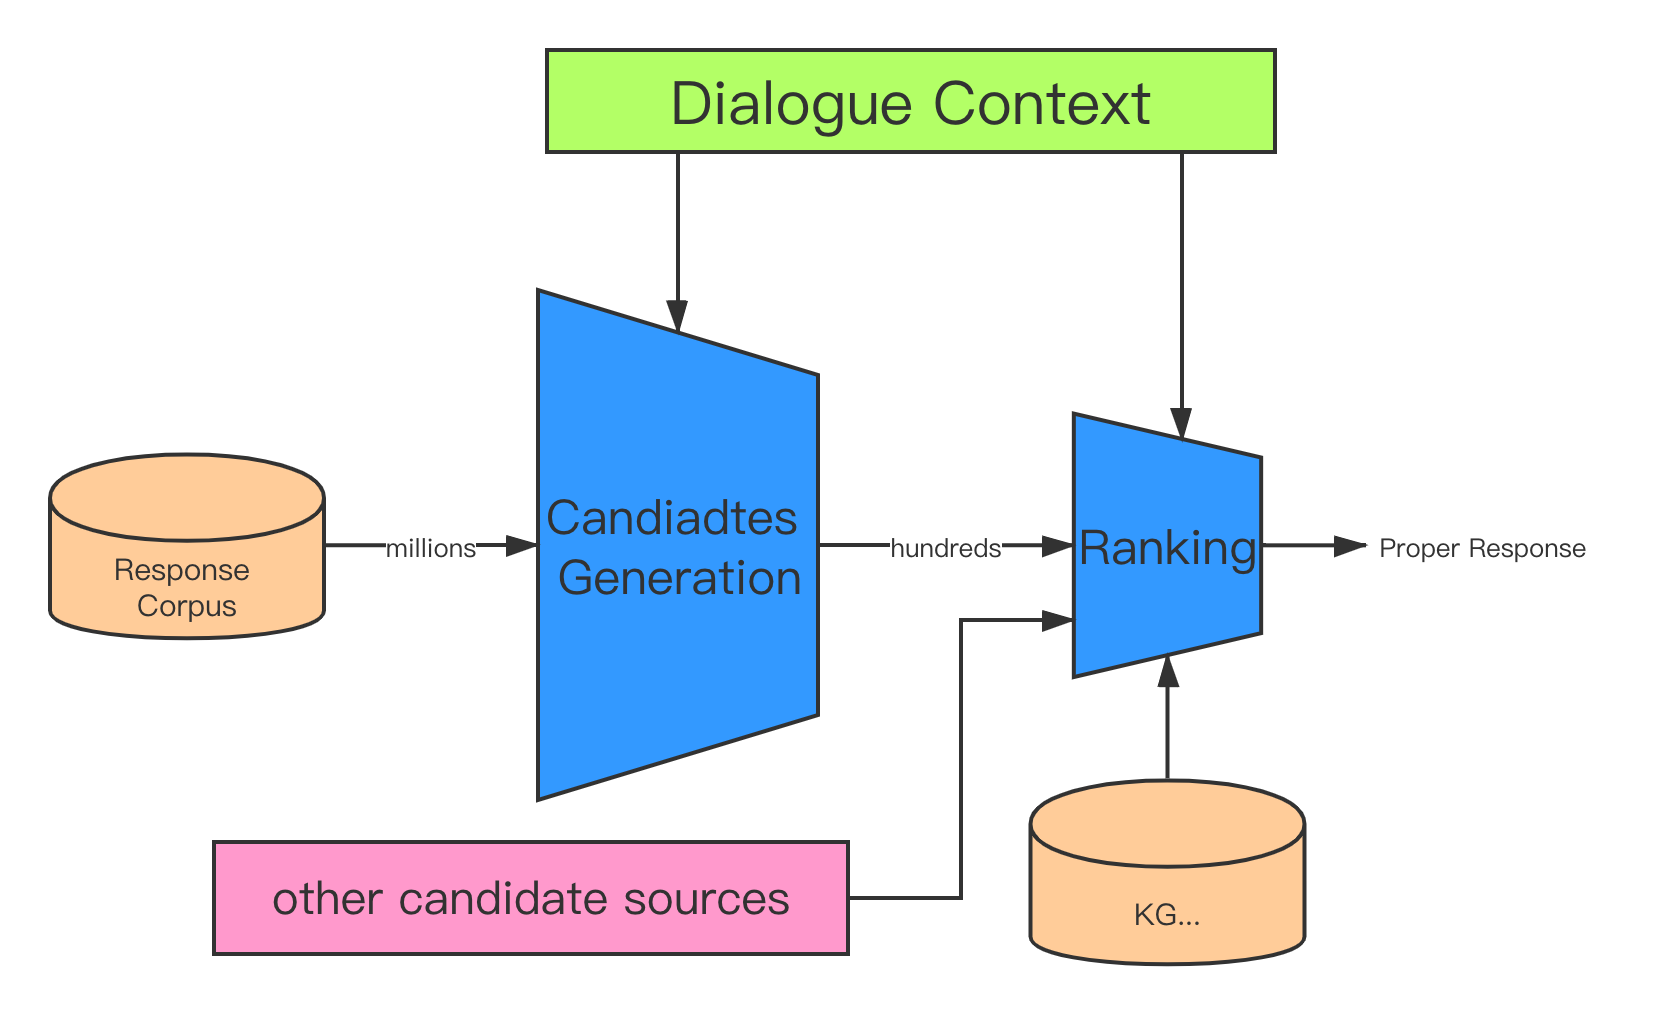
\includegraphics[width=0.8\linewidth]{images/arch.png}
	\label{figure1}
\end{figure}

\section{NLP in General Dialog System}
\label{section3}

\subsection{Dialog System Architecture}

Now dialog systems are typically implemented using an end-to-end architecture, rather than a modular architecture in academic settings because we pursue higher matching score, besides they may test on a small candidate test set instead of using a common huge candidate set. This is unreasonable to show the power of their model. So when we have a huge candidate corpus, a multi-stage recall system is better to use in reality. We give a common architecture similar to Recommend System in figure \ref{figure1}.

The architecture consists of three main part: 1) Response Corpus, a pre-collected well-prepared datasets with high-quality hand-constructed Responses. 2) Candidate Generation System, a coarse-grained selection module recalls a candidate set of responses that are semantic coherent with the conversation context from the pre-constructed database. 3) Ranking System, a fine-grained selection module selects the most appropriate one as the final response to the given conversation context based on the candidate set provided by the Candidate Generation System. Other module such as Knowledge Graph also can been add into this framework, which can help improve these selection module.

\subsection{Ranking System Module}

In a retrieval-based dialog system, the fine-grained selection module part has been greatly researched. These modern neural models of fine-grained match models can be roughly grouped into two categories by \cite{huang2020challenges}: shallow and deep interaction networks. In shallow interaction network, the feature vectors of input and candidate are obtained independently, and there may be shallow interactions such as subtraction or element-wise multiplication between the two vectors before the classification layer. In deep interaction network, the input and candidate make interactions in the early stage to obtain a feature vector for the classification layer.

We show the frameworks of shallow and deep interaction networks, which is drew by \cite{huang2020challenges}:

\begin{figure}[htb]
\caption{Frameworks of shallow and deep interaction networks}
	\centering
	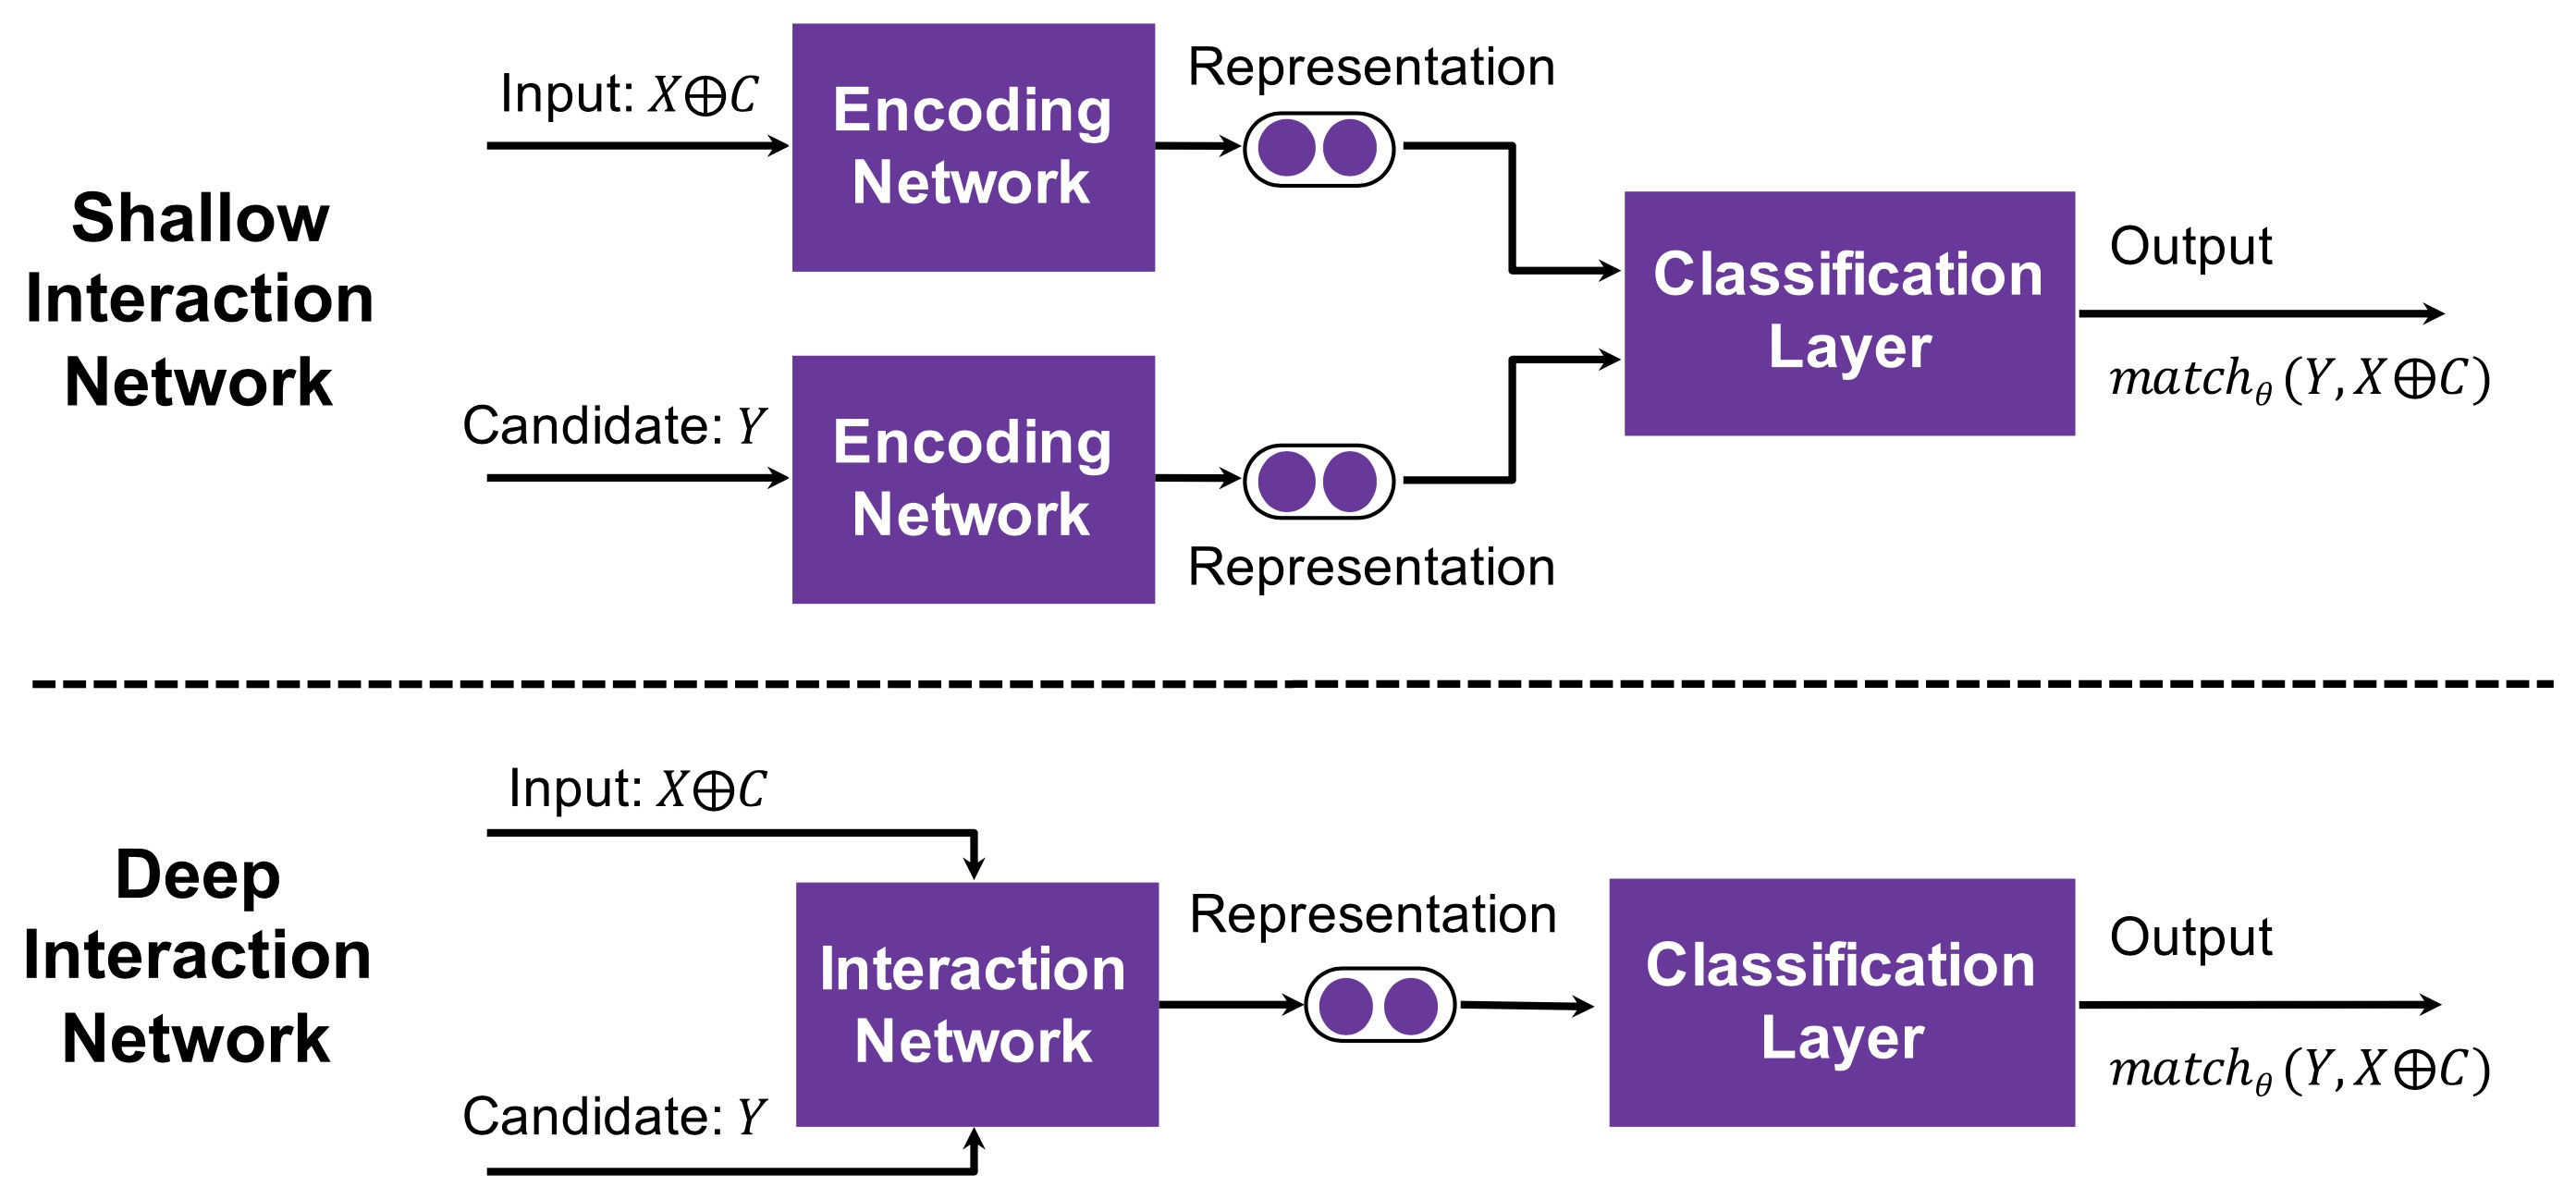
\includegraphics[width=1\linewidth]{images/Frameworks of shallow and deep interaction networks.png}
	\label{fig:fig1}
\end{figure}

Shallow Interaction Network such as Bi-Encoder(\cite{humeau2019poly}) uses Bert(\cite{devlin2018bert}) as Encoding Network and get the Context Representation and Candidate Representation and calculate their dot product or cosine similarity as matching score while Deep Interaction Network such as Cross-Encoder(\cite{humeau2019poly}) concatenate Context and Candidate and send into Bert Interaction Network which has several transformer modules help get deep interaction to get merged Representation and use simple Multi Linear Layers as Classification Layer. \cite{urbanek2019learning} finds that the Deep Interaction Network performs better than Shallow Interaction Network while the performance gains come at a steep computational cost. As we can see, the candidate corpus is fixed in a period of time, so we can save the candidate representation locally. This will help reduce most of encoding time. Now there exists many research work on how to reduce time on candidate and input encoding and can get better interaction between input and candidate. \cite{humeau2019poly} proposed Poly-Encoder learns global rather than token level self-attention features and can faster than Cross-encoders and more accurate than Bi-encoders.They mainly use candidate representation to do global attention between context and candidate to get context representation. The SOTA(state of the art) methods today are basically based on transformer modules, that is to say they is similar to the model before. Although use Bert as Encoding Network can get a better performance, but the inference speed time will increase especially without the computing acceleration of GPU. So when in production environment, easy encoding modules such as LSTM, CNN are more popular for their low cost and superior inference speed. A typical representative is ESIM(\cite{chen2019sequential}), use Bi-LSTM with multi-head self-attention pooling, ranks the top in the DSTC7(\cite{gunasekara2019dstc7}) challenge.

For these neural-based models, they are mainly based on back-propagation algorithm such as Adam(\cite{kingma2014adam}) to update the parameters in the network. So for these models, two loss functions are mainly calculated:
\paragraph{Binary Cross Entropy} is a measure of the difference between two probability distributions over the same underlying set of events which is often used in classification problems.

\begin{equation}
{\mathcal {L}}(X, Y)=-\left[Y \cdot \log X+\left(1-Y \right) \cdot \log \left(1-X\right)\right]
\end{equation}

and the X, Y independently means predict probability distributions and true probability distributions.

\paragraph{Triplet Loss} one of traditional learning-to-rank algorithms, where a baseline input is compared to a positive input and a negative input. The distance from the baseline input to the positive input is minimized, and the distance from the baseline input to the negative input is maximized.

\begin{equation}
{\displaystyle {\mathcal {L}}\left(A,P,N\right)=\operatorname {max} \left({\operatorname{d} (\operatorname {f} \left(A\right)-\operatorname {f} \left(P\right)})-\operatorname{d}({\operatorname {f} \left(A\right)-\operatorname {f} \left(N\right)})+\alpha ,0\right)}
    % \mathcal{L}=\max \left(0, \gamma+\operatorname{match}_{\theta}\left(Y_{-}, X \oplus C\right)-\operatorname{match}_{\theta}\left(Y_{+}, X \oplus C\right)\right)
\end{equation}

and $A$ is a baseline input(context), $P$ is positive input(true response), $N$ is negative input(false response). $f$ here is the function of encoding network instead. $d$ is distance function and cosine distance is a commonly used distance function for its' low computing cost and good spatial properties(capacity to be transformed into ANN problems). $\alpha$ is margin, a parameter that needs to be set in advance, which controls the distance difference between $P$ and $N$ with $A$ to meet a certain interval.

\subsection{Candidate Generation System Module}

\begin{table}[htb]
\caption{Results of Recall@k and human evaluation for random, frequency, and clustering whitelists of different sizes. The “+” indicates that the true response is added to the whitelist.}
\begin{tabular}{|c|c|c|c|c|c|}
\hline Whitelist & $\mathbf{R} @ \mathbf{1}$ & $\mathbf{R} @ \mathbf{3}$ & $\mathbf{R} @ \mathbf{5}$ & $\mathbf{R} @ \mathbf{1 0}$ & $\mathbf{B L E U}$ \\
\hline Random 10K+ & 0.252 & 0.400 & 0.472 & 0.560 & 37.71 \\
Frequency 10K+ & 0.257 & 0.389 & 0.455 & 0.544 & 41.34 \\
Clustering 10K+ & 0.230 & 0.376 & 0.447 & 0.541 & 37.59 \\
\hline Random 1K+ & 0.496 & 0.663 & 0.728 & 0.805 & 59.28 \\
Frequency 1K+ & 0.513 & 0.666 & 0.726 & 0.794 & 67.05 \\
Clustering 1K+ & 0.481 & 0.667 & 0.745 & 0.835 & 61.88 \\
\hline \hline Frequency 10K & 0.136 & 0.261 & 0.327 & 0.420 & 30.46 \\
Clustering 10K & 0.164 & 0.292 & 0.360 & 0.457 & 31.47 \\
\hline Frequency 1K & 0.273 & 0.465 & 0.550 & 0.658 & 47.13 \\
Clustering 1K & 0.331 & 0.542 & 0.650 & 0.782 & 49.26 \\
\hline
\end{tabular}
\begin{tabular}{|c|c|c|c|c|}
\hline \text { Whitelist } & \text { Great } & \text { Good } & \text { Bad } & \text { Accept } \\
\hline \text { Freq. 1K } & 54 \% & 26 \% & 20 \% & 80 \% \\
\text { Cluster. 1K } & 55 \% & 21 \% & 23 \% & 77 \% \\
\text { Freq. 10K } & 56 \% & 24 \% & 21 \% & 80 \% \\
\text { Cluster. 10K } & 57 \% & 23 \% & 20 \% & 80 \% \\
\hline \text { Real response } & 60 \% & 24 \% & 16 \% & 84 \% \\
\hline
\end{tabular}
    \label{table1}
\end{table}

For Candidates Generation Systems, few work are researched in this area. \cite{swanson2019building} have done some research on Candidates Generation. They use three methods to generate a smaller set of candidates($N$ responses), namely:

\begin{itemize}
	\item \textbf{Random Whitelist}: extract N responses randomly from response corpus
	\item \textbf{Frequency Whitelist}: select N common agent responses, after accounting for minor variations in capitalization, punctuation, and whitespace for responses that are sent frequently are more likely to be relevant in multiple conversations and are less likely to contain errors.
	\item \textbf{Clustering Whitelist}: encode all agent responses using response encoder and then used k-means clustering with $k=N$ to cluster the responses and then selected the most common response from each cluster to create the whitelists to help remove many redundant responses.
\end{itemize}

They compute recall when the true response is added to the whitelist and BLEU scores between the true responses and the best suggested responses. To make the assessment more convincing, they also conducted a human evaluation. We compiled their experimental results and presented them for in-depth analysis in Table \ref{table1}. From the Table \ref{table1} left side, we can see that use frequency-based method to construct a candidate set is better than other method if we can know the all true positive response in advance. However it is unrealistic, so a clustering whitelist may be preferred more. We also can see though in recall metric frequency whitelist without gound-truth performs worse than clustering whitelist with same size, it's actual effect is similar to clustering whitelist's in the Table \ref{table1} right side. Above all, the main ideas of these methods are based on filtering out the responses with similar semantics to reduce the size of the candidate set, but we believe that these responses should not be filtered, and should be entered as part of the fine-grained ranking system for next comparison.

Except this, in challenge DSTC7, \cite{chen2019sequential} uses a fast fine-grained ranking system to generate candidate set, but the final result is very general. Considering the accuracy of their shallow interaction network ranking system is low, so we conducted some additional experiments to verify in next section.

\section{Experiment and Analysis}

\subsection{Retrieval Experiment}

Unlike before, we use a more precise method to carry out the experiment. We use the encoder in pre-trained Bi-Encoder model to encode all responses in response corpus to get all response representation offline and save it on the local disk as a tensor. In Bi-Encoder we use cosine similarity as score, so the more similar semantically between context and response, the closer between context representation and response representation. Vice versa. So we can transform a ranking problem to get top-k candidates to a k-nearest neighbors problem. This is a great optimization because as we all know a common method like k-dimension tree with refactoring function like Scapegoat tree has $O(\log n)$ time complexity of insert/delete. We use faiss(\cite{johnson2019billion}) with ANN algorithm to solve this problem for that it can use GPU to speed up computing. The code is published online: \url{https://github.com/Hu-chi/Retrieval-Based-Chatbot} \space .

We use douban dataset(\cite{wu2016sequential}), which is a popular response selection dataset and contains dialogs crawled from the Douban Group. The dataset has some conversation with zero or multiple ground-truths. We just ignore these cases without ground-truths and keep those cases with multiple ground-truths for their greater value. We test our offline model on douban test dataset and calculate these metric in table \ref{table2}, we have also collected the test results of excellent models in recent years, but these models are all deep interaction network, as following:

\begin{table}[htb]
% See awesome Table~\ref{tab:table}.
	\centering
	\caption{metric of different models on douban dataset}
\begin{tabular}{lllllll}
model & ACC & R1@10 & R5@10 & MRR & P@1 & MAP \\
\hline
 SMN (\cite{wu2016sequential}) & - & 0.233 & 0.724 & 0.569 & 0.397 & 0.529 \\
 DUA (\cite{zhang2018modeling}) & - & 0.243 & 0.780 & 0.599 & 0.421 & 0.551 \\
 DAM (\cite{zhou2018multi}) & - & 0.254 & 0.757 & 0.601 & 0.427 & 0.550 \\
 IoI (\cite{tao2019one}) & - & 0.269 & 0.786 & 0.621 & 0.444 & 0.573 \\
 MSN (\cite{yuan2019multi}) & - & 0.295 & 0.788 & 0.632 & 0.470 & 0.587 \\
 \hline
 Cross-Encoder(\cite{gu2020speaker}) & - & 0.280 & 0.828 & 0.633 & 0.454 & 0.591 \\
 SA-BERT(\cite{gu2020speaker}) & - & 0.313 & 0.847 & 0.659 & 0.496 & 0.619 \\
 $\rm {UMS_{BERT+}}$(\cite{whang2020response}) & - & 0.318 & 0.858 & 0.664 & 0.499 & 0.625 \\
 \hline
 Bi-Encoder & 0.854 & 0.249 & 0.783 & 0.601 & 0.406 & 0.562 \\

\end{tabular}
\label{table2}
\end{table}

The offline model is basic Bi-Encoder Model(shallow interaction network), we use Bert to be encoder which is pre-trained on the Next-Sentence and Mask Language Model tasks with large-scale dataset to obtain better word representation. In practice it has surfaced that transfer learning can have better generalization performance on most NLP tasks.

From table \ref{table2}, we can see that the Bi-Encoder, a shallow interaction network, performs worse than deep interaction network and it's a perfectly normal thing. Bi-Encoder is a coarse-grained selection model, it serves for Candidate Generation Systems. We are more concerned about the speed of retrieval and the recall rate of candidate set. So we continue to conduct this experiment and results in table \ref{table3}.

\begin{table}[htb]
	\caption{Recall for candidate sets with different corpus}
	\centering
	\begin{tabular}{lllllllll}
	\hline
	\text { K: size} & \text { R1@K } & \text { R2@K } & \text { R4@K } & \text { R8@K } & \text { R16@K } & \text { R32@K } & \text { R64@K } & \text { R128@K }  \\
	\hline
	1M & 0.67 \% & 1.01 \% & 1.57 \% & 2.34 \% & 3.45 \% & 5.00
	\% & 7.15 \% & 10.04 \%  \\
	\hline
	500K & 0.89 \% & 1.44 \% & 2.19 \% & 3.26 \% & 4.76 \% & 6.84 \% & 9.66 \% & 13.45 \% \\
	\hline
	\text { K:size} & \text { R256@K } & \text { R512@K } & \text { R1024@K } & \text { R2048@K } & \text { R4096@K } & \text { R5000@K } & \text { R8192@K } &   \\
	\hline
	1M & 13.93\% & 19.05\%	& 25.49\%	& 33.58\% &43.34\%  & - & -
	\\ \hline
	500K & 18.48\%	& 24.84\%&	32.88\% &	42.59\% & 53.77\%	&57.15\%&	65.74\% \\
	\end{tabular}
	\label{table3}
\end{table}

We have made two response corpus, one of which is a one million ordinary dataset composed of half of  positive responses and half of negative responses, and another is a dataset composed of only positive examples which has higher quality. The offline model's purpose is to generated candidate set dynamically, and we can see from table \ref{table3}, if we generate a 8192 size candidate set, it's Recall rate is only 65.738\% and it seems that its' effect is general. But the metric ignores the other candidates'  contributions on semantic similarity as we talked about before. After all each one context has just only one ground-truth during testing, other candidates are considered negative cases, which is not realistic under large dataset.

Another metric we care about is inference speed, the time cost for generating candidate set. The time for generating candidate set can be divided into three parts: 1) the encoding time for context, 2) the encoding time for all candidates in corpus, 3) recall candidates from corpus to generate candidate set. For first part, \cite{humeau2019poly} has evaluated this, they predict the next utterance for 100 dialogue examples in the ConvAI2 validation set with both CPU-only and GPU setups. For CPU-only, they use an 80 core Intel Xeon processor CPU E5-2698. For GPU setups, they use a single Nvidia Quadro GP100 using cuda 10.0 and cudnn 7.4. The results are in the table \ref{table4}.

\begin{table}[htb]
\caption{inference time for encoding}
    \centering
    \begin{tabular}{|c|c|c|c|c|}
\hline & \multicolumn{4}{|c|} { Scoring time (ms) }  \\
\hline & \multicolumn{2}{|c|} { CPU } & \multicolumn{2}{c|} { GPU } \\
\hline Candidates & $1 \mathrm{k}$ & $100 \mathrm{k}$ & $1 \mathrm{k}$ & $100 \mathrm{k}$ \\
\hline \hline Bi-encoder & 115 & 160 & 19 & 22 \\
\hline Poly-encoder & 160 & 837 & 57 & 88 \\
\hline Cross-encoder & $21.7 \mathrm{k}$ & $2.2 \mathrm{M}^{*}$ & $2.6 \mathrm{k}$ & $266 \mathrm{k}^{*}$ \\
\hline
\end{tabular}
    \label{table4}
\end{table}

For second part, the encoding time for all candidates in corpus is obviously huge, but it only needs to be executed once in advance, so it doesn't cost time during inference. And for the last part about recalling with ANN algorithm, with faiss library's help, we test it on Douban dataset. When we recall 4096 candidate set from 1 Million corpus, it only costs time 250ms on CPU-only or 10ms on GPU. We can deploy the model on distributed streaming systems such as Storm, which can be used in industrial scenarios.
% \cite{swanson2019building}

\subsection{System Analysis}

Retrieval-based dialog systems have been extensively researched in the past few years. Since transfer learning with large corpus, pre-training models have been widely used in NLP area, its' performance is now difficult to improve greatly. At present,\cite{henderson2019convert} use larger dataset such as Reddit to obtain utterance representations that are more suitable for dialog retrieval task, but these are time-consuming and costly, and the improvements they bring are limited. The final models are also very huge. In addition, \cite{xu2020learning} modify pre-training tasks to help obtain better representations. However, we believe that current work is overly dependent on pre-trained models such as Bert, and ignores the unique task attributes of dialog-related tasks. The previous model that used to design the RNN model to track state changes in the dialog also performed well, but it could not get better results based on the pre-trained model. We think one solution is to learn better parameters through multi-tasking learning. For example, we can combine emotion recognition in conversation, dialog intention recognition and other tasks. These tasks are all related to dialog and need to pay attention to the underlying structure in the dialog. Multi-task learning can better optimize model parameters from different angles. However, the current problem is that there is no relevant dataset that can be applied.

If we want to continue to apply the retrieval-based dialog system into production, then the problem that needs to be solved is how to reduce the size of response corpus. Although the current candidate set can be stored in a distributed system, it is still not a wise move. From a certain point of view,  utterances with highly similar semantics are redundant information. We need to find meta-response and generate better and more similar response through meta-response. We can incorporate knowledge from knowledge graph into  generation process, also including other factors such as emotion, personality. And our candidate set should only contains meta-replies. This will greatly reduce the space occupied by the stored data, and can be more applicable in many small scenarios. In addition, we can also reduce the space occupied by the corpus by means of knowledge distillation, vector quantization, and reduction of the representation dimension, but this is not a breakthrough. \cite{lan2020ultra} have done this work recently, but it also brings performance degradation.

\section{Conclusion}

At present, we have discussed a lot about retrieval-based dialog systems, but do not give an end-to-end neural-based solution, because this is obviously not feasible on large dataset. If you need to build an end-to-end solution, a better approach is to choose a generation-based dialog system model, but we still cannot control the generated content at this stage, so whether the generated content is legally required and whether it meets the bottom line of society still needs follow-up processing. It is due to learning a lot of vulgar conversations on the Internet, which leads to the final failure of Microsoft project Tay, and should arouse our vigilance.

In the background of our above system, we default that all conversations are pure text, but now, with the popularity of emoji, more and more stickers appear in our usual conversations. In addition, there are various Multi-modal information, and even multi-lingual dialog, have brought great difficulties to the current dialog system, but at the same time it is also worth pondering over what a more complete dialog system should do. At present, \cite{gao2020learning} do a research on retrieving stickers in the dialogue, but their tasks are too simple to be practically used in production scenarios. A dialog system with better robustness must be our next step.

As a bridge between humans and machines, the dialog system can be easily combined with other tasks, such as information retrieval systems, recommendation systems, language assistants, etc. With the continuous development of the dialogue system, we believe that its ultimate success will cause a huge change in human life style.

\bibliographystyle{unsrtnat}
\bibliography{references}

\end{document}
